% Options for packages loaded elsewhere
\PassOptionsToPackage{unicode}{hyperref}
\PassOptionsToPackage{hyphens}{url}
%
\documentclass[
]{article}
\usepackage{amsmath,amssymb}
\usepackage{iftex}
\ifPDFTeX
  \usepackage[T1]{fontenc}
  \usepackage[utf8]{inputenc}
  \usepackage{textcomp} % provide euro and other symbols
\else % if luatex or xetex
  \usepackage{unicode-math} % this also loads fontspec
  \defaultfontfeatures{Scale=MatchLowercase}
  \defaultfontfeatures[\rmfamily]{Ligatures=TeX,Scale=1}
\fi
\usepackage{lmodern}
\ifPDFTeX\else
  % xetex/luatex font selection
\fi
% Use upquote if available, for straight quotes in verbatim environments
\IfFileExists{upquote.sty}{\usepackage{upquote}}{}
\IfFileExists{microtype.sty}{% use microtype if available
  \usepackage[]{microtype}
  \UseMicrotypeSet[protrusion]{basicmath} % disable protrusion for tt fonts
}{}
\makeatletter
\@ifundefined{KOMAClassName}{% if non-KOMA class
  \IfFileExists{parskip.sty}{%
    \usepackage{parskip}
  }{% else
    \setlength{\parindent}{0pt}
    \setlength{\parskip}{6pt plus 2pt minus 1pt}}
}{% if KOMA class
  \KOMAoptions{parskip=half}}
\makeatother
\usepackage{xcolor}
\usepackage[margin=1in]{geometry}
\usepackage{color}
\usepackage{fancyvrb}
\newcommand{\VerbBar}{|}
\newcommand{\VERB}{\Verb[commandchars=\\\{\}]}
\DefineVerbatimEnvironment{Highlighting}{Verbatim}{commandchars=\\\{\}}
% Add ',fontsize=\small' for more characters per line
\usepackage{framed}
\definecolor{shadecolor}{RGB}{248,248,248}
\newenvironment{Shaded}{\begin{snugshade}}{\end{snugshade}}
\newcommand{\AlertTok}[1]{\textcolor[rgb]{0.94,0.16,0.16}{#1}}
\newcommand{\AnnotationTok}[1]{\textcolor[rgb]{0.56,0.35,0.01}{\textbf{\textit{#1}}}}
\newcommand{\AttributeTok}[1]{\textcolor[rgb]{0.13,0.29,0.53}{#1}}
\newcommand{\BaseNTok}[1]{\textcolor[rgb]{0.00,0.00,0.81}{#1}}
\newcommand{\BuiltInTok}[1]{#1}
\newcommand{\CharTok}[1]{\textcolor[rgb]{0.31,0.60,0.02}{#1}}
\newcommand{\CommentTok}[1]{\textcolor[rgb]{0.56,0.35,0.01}{\textit{#1}}}
\newcommand{\CommentVarTok}[1]{\textcolor[rgb]{0.56,0.35,0.01}{\textbf{\textit{#1}}}}
\newcommand{\ConstantTok}[1]{\textcolor[rgb]{0.56,0.35,0.01}{#1}}
\newcommand{\ControlFlowTok}[1]{\textcolor[rgb]{0.13,0.29,0.53}{\textbf{#1}}}
\newcommand{\DataTypeTok}[1]{\textcolor[rgb]{0.13,0.29,0.53}{#1}}
\newcommand{\DecValTok}[1]{\textcolor[rgb]{0.00,0.00,0.81}{#1}}
\newcommand{\DocumentationTok}[1]{\textcolor[rgb]{0.56,0.35,0.01}{\textbf{\textit{#1}}}}
\newcommand{\ErrorTok}[1]{\textcolor[rgb]{0.64,0.00,0.00}{\textbf{#1}}}
\newcommand{\ExtensionTok}[1]{#1}
\newcommand{\FloatTok}[1]{\textcolor[rgb]{0.00,0.00,0.81}{#1}}
\newcommand{\FunctionTok}[1]{\textcolor[rgb]{0.13,0.29,0.53}{\textbf{#1}}}
\newcommand{\ImportTok}[1]{#1}
\newcommand{\InformationTok}[1]{\textcolor[rgb]{0.56,0.35,0.01}{\textbf{\textit{#1}}}}
\newcommand{\KeywordTok}[1]{\textcolor[rgb]{0.13,0.29,0.53}{\textbf{#1}}}
\newcommand{\NormalTok}[1]{#1}
\newcommand{\OperatorTok}[1]{\textcolor[rgb]{0.81,0.36,0.00}{\textbf{#1}}}
\newcommand{\OtherTok}[1]{\textcolor[rgb]{0.56,0.35,0.01}{#1}}
\newcommand{\PreprocessorTok}[1]{\textcolor[rgb]{0.56,0.35,0.01}{\textit{#1}}}
\newcommand{\RegionMarkerTok}[1]{#1}
\newcommand{\SpecialCharTok}[1]{\textcolor[rgb]{0.81,0.36,0.00}{\textbf{#1}}}
\newcommand{\SpecialStringTok}[1]{\textcolor[rgb]{0.31,0.60,0.02}{#1}}
\newcommand{\StringTok}[1]{\textcolor[rgb]{0.31,0.60,0.02}{#1}}
\newcommand{\VariableTok}[1]{\textcolor[rgb]{0.00,0.00,0.00}{#1}}
\newcommand{\VerbatimStringTok}[1]{\textcolor[rgb]{0.31,0.60,0.02}{#1}}
\newcommand{\WarningTok}[1]{\textcolor[rgb]{0.56,0.35,0.01}{\textbf{\textit{#1}}}}
\usepackage{graphicx}
\makeatletter
\def\maxwidth{\ifdim\Gin@nat@width>\linewidth\linewidth\else\Gin@nat@width\fi}
\def\maxheight{\ifdim\Gin@nat@height>\textheight\textheight\else\Gin@nat@height\fi}
\makeatother
% Scale images if necessary, so that they will not overflow the page
% margins by default, and it is still possible to overwrite the defaults
% using explicit options in \includegraphics[width, height, ...]{}
\setkeys{Gin}{width=\maxwidth,height=\maxheight,keepaspectratio}
% Set default figure placement to htbp
\makeatletter
\def\fps@figure{htbp}
\makeatother
\setlength{\emergencystretch}{3em} % prevent overfull lines
\providecommand{\tightlist}{%
  \setlength{\itemsep}{0pt}\setlength{\parskip}{0pt}}
\setcounter{secnumdepth}{-\maxdimen} % remove section numbering
\ifLuaTeX
  \usepackage{selnolig}  % disable illegal ligatures
\fi
\IfFileExists{bookmark.sty}{\usepackage{bookmark}}{\usepackage{hyperref}}
\IfFileExists{xurl.sty}{\usepackage{xurl}}{} % add URL line breaks if available
\urlstyle{same}
\hypersetup{
  pdftitle={Statistical Computing},
  pdfauthor={Tinotenda Mutsemi},
  hidelinks,
  pdfcreator={LaTeX via pandoc}}

\title{Statistical Computing}
\usepackage{etoolbox}
\makeatletter
\providecommand{\subtitle}[1]{% add subtitle to \maketitle
  \apptocmd{\@title}{\par {\large #1 \par}}{}{}
}
\makeatother
\subtitle{Assignment 2}
\author{Tinotenda Mutsemi}
\date{2024-03-05}

\begin{document}
\maketitle

\begin{Shaded}
\begin{Highlighting}[]
\FunctionTok{library}\NormalTok{(dplyr)}
\end{Highlighting}
\end{Shaded}

\begin{verbatim}
## 
## Attaching package: 'dplyr'
\end{verbatim}

\begin{verbatim}
## The following objects are masked from 'package:stats':
## 
##     filter, lag
\end{verbatim}

\begin{verbatim}
## The following objects are masked from 'package:base':
## 
##     intersect, setdiff, setequal, union
\end{verbatim}

\begin{Shaded}
\begin{Highlighting}[]
\FunctionTok{library}\NormalTok{(ggplot2)}
\FunctionTok{library}\NormalTok{(xlsx)}
\end{Highlighting}
\end{Shaded}

\begin{verbatim}
## Warning: package 'xlsx' was built under R version 4.3.3
\end{verbatim}

\begin{Shaded}
\begin{Highlighting}[]
\FunctionTok{library}\NormalTok{(reshape2)}
\end{Highlighting}
\end{Shaded}

\begin{Shaded}
\begin{Highlighting}[]
\CommentTok{\#read data}
\NormalTok{lex\_raw }\OtherTok{\textless{}{-}} \FunctionTok{read.csv}\NormalTok{(}\StringTok{"lex.csv"}\NormalTok{)}
\NormalTok{gdp\_pcap\_raw }\OtherTok{\textless{}{-}} \FunctionTok{read.csv}\NormalTok{(}\StringTok{"gdp\_pcap.csv"}\NormalTok{)}
\NormalTok{region\_raw }\OtherTok{\textless{}{-}} \FunctionTok{read.xlsx}\NormalTok{(}\StringTok{"Data Geographies {-} v2 {-} by Gapminder.xlsx"}\NormalTok{, }\AttributeTok{sheetIndex =} \DecValTok{2}\NormalTok{)}
\NormalTok{population\_raw }\OtherTok{\textless{}{-}} \FunctionTok{read.xlsx}\NormalTok{(}\StringTok{"GM{-}Population {-} Dataset {-} v6.xlsx"}\NormalTok{, }\AttributeTok{sheetIndex =} \DecValTok{4}\NormalTok{)}
\end{Highlighting}
\end{Shaded}

\begin{Shaded}
\begin{Highlighting}[]
\CommentTok{\#Qtn 1a}
\CommentTok{\#data cleaning and selcting required data}
\NormalTok{lex\_2019 }\OtherTok{\textless{}{-}} \FunctionTok{select}\NormalTok{(lex\_raw, country, X2019)}

\NormalTok{gdp\_pcap\_2019 }\OtherTok{\textless{}{-}} \FunctionTok{select}\NormalTok{(gdp\_pcap\_raw, country, X2019)}

\CommentTok{\#region data}
\CommentTok{\#rename region col names}
\NormalTok{lookup }\OtherTok{\textless{}{-}} \FunctionTok{c}\NormalTok{(}\AttributeTok{country =} \StringTok{"name"}\NormalTok{,}
            \AttributeTok{region =} \StringTok{"four\_regions"}\NormalTok{)}
\NormalTok{region }\OtherTok{\textless{}{-}} \FunctionTok{select}\NormalTok{(region\_raw, name, four\_regions) }\SpecialCharTok{|\textgreater{}} \FunctionTok{rename}\NormalTok{(}\FunctionTok{all\_of}\NormalTok{(lookup))}


\CommentTok{\#population data}
\CommentTok{\#deselect col}
\NormalTok{population\_raw2 }\OtherTok{\textless{}{-}} \FunctionTok{select}\NormalTok{(population\_raw, }\SpecialCharTok{{-}}\NormalTok{geo)}
\CommentTok{\#rename cols}
\NormalTok{lookup }\OtherTok{\textless{}{-}} \FunctionTok{c}\NormalTok{(}\AttributeTok{country =} \StringTok{"name"}\NormalTok{,}
            \AttributeTok{year =} \StringTok{"time"}\NormalTok{,}
            \AttributeTok{population =} \StringTok{"Population"}\NormalTok{)}

\NormalTok{population\_raw2 }\OtherTok{\textless{}{-}} \FunctionTok{rename}\NormalTok{(population\_raw2, }\FunctionTok{all\_of}\NormalTok{(lookup))}

\CommentTok{\#select 2019 population}
\NormalTok{population\_2019 }\OtherTok{\textless{}{-}} \FunctionTok{filter}\NormalTok{(population\_raw2, year }\SpecialCharTok{==} \DecValTok{2019}\NormalTok{)}
\end{Highlighting}
\end{Shaded}

\begin{Shaded}
\begin{Highlighting}[]
\CommentTok{\#merge and clean data frames}
\NormalTok{lex\_gdp\_2019 }\OtherTok{\textless{}{-}} \FunctionTok{full\_join}\NormalTok{(lex\_2019, gdp\_pcap\_2019, }\AttributeTok{by =} \FunctionTok{join\_by}\NormalTok{(country))}
\NormalTok{lex\_gdp\_region\_2019 }\OtherTok{\textless{}{-}} \FunctionTok{full\_join}\NormalTok{(lex\_gdp\_2019, region, }\AttributeTok{by =} \FunctionTok{join\_by}\NormalTok{(country))}

\CommentTok{\#rename cols of new df}
\NormalTok{lookup }\OtherTok{\textless{}{-}} \FunctionTok{c}\NormalTok{(}\AttributeTok{lex =} \StringTok{"X2019.x"}\NormalTok{, }
            \AttributeTok{gdp\_pcap =} \StringTok{"X2019.y"}\NormalTok{)}
\NormalTok{lex\_gdp\_region\_2019 }\OtherTok{\textless{}{-}} \FunctionTok{rename}\NormalTok{(lex\_gdp\_region\_2019, }\FunctionTok{all\_of}\NormalTok{(lookup))}

\CommentTok{\#make gdp\_pcap numeric}
\NormalTok{lex\_gdp\_region\_2019}\SpecialCharTok{$}\NormalTok{gdp\_pcap }\OtherTok{\textless{}{-}} \FunctionTok{as.numeric}\NormalTok{(lex\_gdp\_region\_2019}\SpecialCharTok{$}\NormalTok{gdp\_pcap)}
\end{Highlighting}
\end{Shaded}

\begin{verbatim}
## Warning: NAs introduced by coercion
\end{verbatim}

\begin{Shaded}
\begin{Highlighting}[]
\NormalTok{lex\_gdp\_region\_popu\_2019 }\OtherTok{\textless{}{-}} \FunctionTok{full\_join}\NormalTok{(lex\_gdp\_region\_2019, population\_2019, }\AttributeTok{by =} \FunctionTok{join\_by}\NormalTok{(country))}
\end{Highlighting}
\end{Shaded}

\begin{Shaded}
\begin{Highlighting}[]
\NormalTok{plot\_lex\_gdp\_region\_popu\_2019 }\OtherTok{\textless{}{-}} \FunctionTok{na.omit}\NormalTok{(lex\_gdp\_region\_popu\_2019)}
\CommentTok{\#scatter plot with ggplot}
\FunctionTok{ggplot}\NormalTok{(}\AttributeTok{data =}\NormalTok{ plot\_lex\_gdp\_region\_popu\_2019, }\AttributeTok{mapping =} \FunctionTok{aes}\NormalTok{(}\AttributeTok{x =}\NormalTok{ gdp\_pcap, }\AttributeTok{y =}\NormalTok{ lex,}
             \AttributeTok{colour =}\NormalTok{ region,}
             \AttributeTok{size =}\NormalTok{ population,}
\NormalTok{             )) }\SpecialCharTok{+}
  \FunctionTok{geom\_point}\NormalTok{() }\SpecialCharTok{+}
  \FunctionTok{geom\_text}\NormalTok{(}\FunctionTok{aes}\NormalTok{(}\AttributeTok{label =}\NormalTok{ country), }\AttributeTok{check\_overlap =} \ConstantTok{TRUE}\NormalTok{, }\AttributeTok{vjust =} \DecValTok{1}\NormalTok{, }\AttributeTok{hjust =} \DecValTok{1}\NormalTok{, }\AttributeTok{col =} \StringTok{"black"}\NormalTok{) }\SpecialCharTok{+}
  \FunctionTok{scale\_x\_log10}\NormalTok{() }\SpecialCharTok{+}
  \FunctionTok{scale\_y\_log10}\NormalTok{() }\SpecialCharTok{+}
  \FunctionTok{labs}\NormalTok{(}
       \AttributeTok{x =} \StringTok{"GDP per capita"}\NormalTok{,}
       \AttributeTok{y =} \StringTok{"Life expectancy"}\NormalTok{)}
\end{Highlighting}
\end{Shaded}

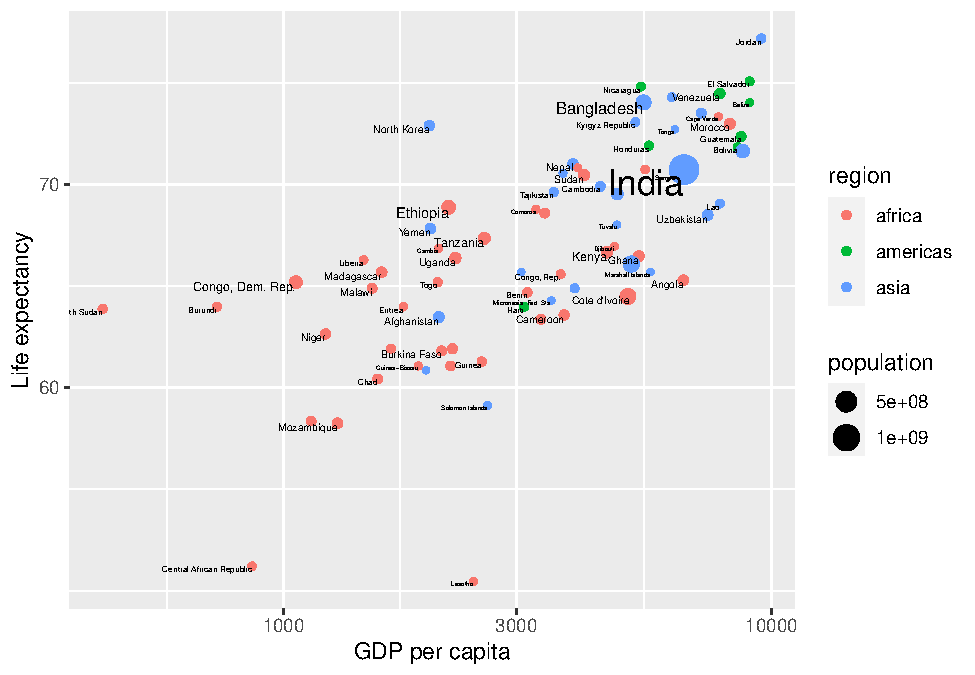
\includegraphics{MTSTIN007_SC_Assingment_2_files/figure-latex/unnamed-chunk-5-1.pdf}

\begin{Shaded}
\begin{Highlighting}[]
  \CommentTok{\# title = "GDP per capita vs Life expectancy 2019",}
\CommentTok{\#save plot}
\FunctionTok{ggsave}\NormalTok{(}\StringTok{"lex\_gdp\_region\_popu\_2019.png"}\NormalTok{)}
\end{Highlighting}
\end{Shaded}

\begin{verbatim}
## Saving 6.5 x 4.5 in image
\end{verbatim}

\begin{Shaded}
\begin{Highlighting}[]
\CommentTok{\#Qtn b}
\NormalTok{region\_avg\_lex }\OtherTok{\textless{}{-}}\NormalTok{ lex\_gdp\_region\_popu\_2019 }\SpecialCharTok{|\textgreater{}} \FunctionTok{group\_by}\NormalTok{(region) }\SpecialCharTok{|\textgreater{}} \FunctionTok{summarise}\NormalTok{(}\AttributeTok{avg\_region\_lex =} \FunctionTok{mean}\NormalTok{(lex, }\AttributeTok{na.rm =} \ConstantTok{TRUE}\NormalTok{), }\AttributeTok{countries\_in\_region =} \FunctionTok{n}\NormalTok{())}

\CommentTok{\#remove na region}
\NormalTok{region\_avg\_lex }\OtherTok{\textless{}{-}} \FunctionTok{na.omit}\NormalTok{(region\_avg\_lex)}

\CommentTok{\#sort by avg\_region\_lex descending}
\NormalTok{region\_avg\_lex }\OtherTok{\textless{}{-}}\NormalTok{ region\_avg\_lex }\SpecialCharTok{|\textgreater{}} \FunctionTok{arrange}\NormalTok{(}\FunctionTok{desc}\NormalTok{(avg\_region\_lex))}
\NormalTok{region\_avg\_lex}
\end{Highlighting}
\end{Shaded}

\begin{verbatim}
## # A tibble: 4 x 3
##   region   avg_region_lex countries_in_region
##   <chr>             <dbl>               <int>
## 1 europe             79.1                  49
## 2 americas           75.2                  35
## 3 asia               73.0                  59
## 4 africa             65.9                  54
\end{verbatim}

\begin{Shaded}
\begin{Highlighting}[]
\CommentTok{\#Qtn c}

\CommentTok{\#melt lex\_raw}
\NormalTok{lex\_melt }\OtherTok{\textless{}{-}} \FunctionTok{melt}\NormalTok{(lex\_raw, }\AttributeTok{id.vars =} \StringTok{"country"}\NormalTok{, }\AttributeTok{value.name =} \StringTok{"lex"}\NormalTok{, }\AttributeTok{variable.name =} \StringTok{"year"}\NormalTok{)}



\CommentTok{\#merge lex\_melt with regions}
\NormalTok{lex\_region }\OtherTok{\textless{}{-}} \FunctionTok{full\_join}\NormalTok{(lex\_melt, region, }\AttributeTok{by =} \StringTok{"country"}\NormalTok{)}

\NormalTok{region\_avg\_lex }\OtherTok{\textless{}{-}}\NormalTok{ lex\_region }\SpecialCharTok{|\textgreater{}} \FunctionTok{group\_by}\NormalTok{(region, year) }\SpecialCharTok{|\textgreater{}} \FunctionTok{summarise}\NormalTok{(}\AttributeTok{avg\_lex =} \FunctionTok{mean}\NormalTok{(lex, }\AttributeTok{na.rm =} \ConstantTok{TRUE}\NormalTok{))}
\end{Highlighting}
\end{Shaded}

\begin{verbatim}
## `summarise()` has grouped output by 'region'. You can override using the
## `.groups` argument.
\end{verbatim}

\begin{Shaded}
\begin{Highlighting}[]
\CommentTok{\#remove leading X from year}
\NormalTok{region\_avg\_lex}\SpecialCharTok{$}\NormalTok{year }\OtherTok{\textless{}{-}} \FunctionTok{gsub}\NormalTok{(}\StringTok{"X"}\NormalTok{, }\StringTok{""}\NormalTok{, region\_avg\_lex}\SpecialCharTok{$}\NormalTok{year)}
\CommentTok{\#make year numeric}
\NormalTok{region\_avg\_lex}\SpecialCharTok{$}\NormalTok{year }\OtherTok{\textless{}{-}} \FunctionTok{as.numeric}\NormalTok{(region\_avg\_lex}\SpecialCharTok{$}\NormalTok{year)}
\end{Highlighting}
\end{Shaded}

\begin{Shaded}
\begin{Highlighting}[]
\NormalTok{plot\_region\_avg\_lex }\OtherTok{=} \FunctionTok{na.omit}\NormalTok{(region\_avg\_lex)}
\FunctionTok{ggplot}\NormalTok{(}\AttributeTok{data =}\NormalTok{ plot\_region\_avg\_lex, }\AttributeTok{mapping =} \FunctionTok{aes}\NormalTok{(}\AttributeTok{x =}\NormalTok{ year, }\AttributeTok{y =}\NormalTok{ avg\_lex, }\AttributeTok{group =}\NormalTok{ region, }\AttributeTok{col =}\NormalTok{ region)) }\SpecialCharTok{+}
  \FunctionTok{geom\_line}\NormalTok{() }\SpecialCharTok{+}
  \FunctionTok{labs}\NormalTok{(}
       \AttributeTok{x =} \StringTok{"Year"}\NormalTok{,}
       \AttributeTok{y =} \StringTok{"Average life expectancy"}\NormalTok{) }\SpecialCharTok{+}
  \FunctionTok{scale\_x\_continuous}\NormalTok{(}\AttributeTok{breaks =} \FunctionTok{seq}\NormalTok{(}\DecValTok{1800}\NormalTok{, }\DecValTok{2160}\NormalTok{,}\DecValTok{20}\NormalTok{)) }\SpecialCharTok{+}
  \FunctionTok{scale\_y\_continuous}\NormalTok{(}\AttributeTok{breaks =} \FunctionTok{seq}\NormalTok{(}\DecValTok{0}\NormalTok{, }\DecValTok{90}\NormalTok{, }\DecValTok{10}\NormalTok{)) }\SpecialCharTok{+}
  \FunctionTok{theme}\NormalTok{(}\AttributeTok{axis.text.x =} \FunctionTok{element\_text}\NormalTok{(}\AttributeTok{angle =} \DecValTok{45}\NormalTok{, }\AttributeTok{vjust =} \FloatTok{0.5}\NormalTok{, }\AttributeTok{hjust =} \DecValTok{1}\NormalTok{))}
\end{Highlighting}
\end{Shaded}

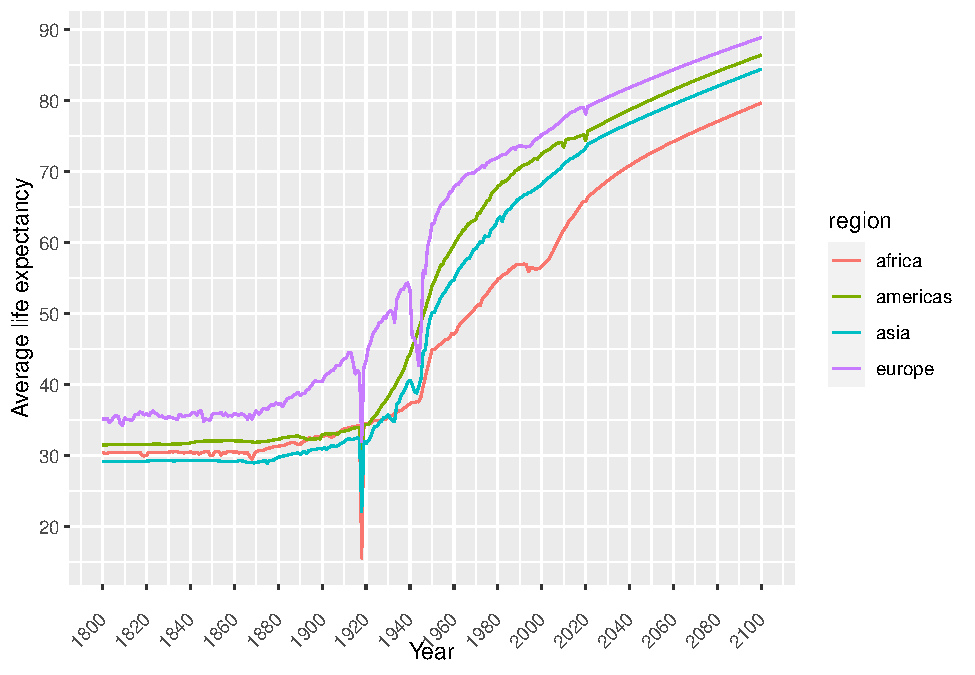
\includegraphics{MTSTIN007_SC_Assingment_2_files/figure-latex/unnamed-chunk-8-1.pdf}

\begin{Shaded}
\begin{Highlighting}[]
\CommentTok{\# title = "Region average life expectancy over time",}

\CommentTok{\#save plot}
\FunctionTok{ggsave}\NormalTok{(}\StringTok{"region\_avg\_lex.png"}\NormalTok{)}
\end{Highlighting}
\end{Shaded}

\begin{verbatim}
## Saving 6.5 x 4.5 in image
\end{verbatim}

\begin{Shaded}
\begin{Highlighting}[]
\CommentTok{\#Qtn d}
\CommentTok{\#select 2019 data}
\NormalTok{region\_avg\_lex\_2019 }\OtherTok{\textless{}{-}} \FunctionTok{filter}\NormalTok{(region\_avg\_lex, year }\SpecialCharTok{==} \DecValTok{2019}\NormalTok{)}
\CommentTok{\#drop na region}
\NormalTok{region\_avg\_lex\_2019 }\OtherTok{\textless{}{-}} \FunctionTok{na.omit}\NormalTok{(region\_avg\_lex\_2019)}

\CommentTok{\#plot bar chart}
\FunctionTok{ggplot}\NormalTok{(}\AttributeTok{data =}\NormalTok{ region\_avg\_lex\_2019, }\AttributeTok{mapping =} \FunctionTok{aes}\NormalTok{(}\AttributeTok{x =}\NormalTok{ region, }\AttributeTok{y =}\NormalTok{ avg\_lex)) }\SpecialCharTok{+}
  \FunctionTok{geom\_bar}\NormalTok{(}\AttributeTok{stat =} \StringTok{"identity"}\NormalTok{) }\SpecialCharTok{+}
  \FunctionTok{labs}\NormalTok{(}
       \AttributeTok{x =} \StringTok{"Region"}\NormalTok{,}
       \AttributeTok{y =} \StringTok{"Average life expectancy"}\NormalTok{) }\SpecialCharTok{+}
  \CommentTok{\# theme(axis.text.x = element\_text(angle = 45, vjust = 0.5, hjust = 1)) +}
  \FunctionTok{scale\_y\_continuous}\NormalTok{(}\AttributeTok{breaks =} \FunctionTok{seq}\NormalTok{(}\DecValTok{0}\NormalTok{, }\DecValTok{90}\NormalTok{, }\DecValTok{10}\NormalTok{)) }\SpecialCharTok{+}
  \FunctionTok{geom\_text}\NormalTok{(}\FunctionTok{aes}\NormalTok{(}\AttributeTok{label =} \FunctionTok{round}\NormalTok{(avg\_lex, }\DecValTok{0}\NormalTok{)), }\AttributeTok{vjust =} \SpecialCharTok{{-}}\FloatTok{0.5}\NormalTok{, }\AttributeTok{hjust =} \DecValTok{1}\NormalTok{, }\AttributeTok{col =} \StringTok{"black"}\NormalTok{)}
\end{Highlighting}
\end{Shaded}

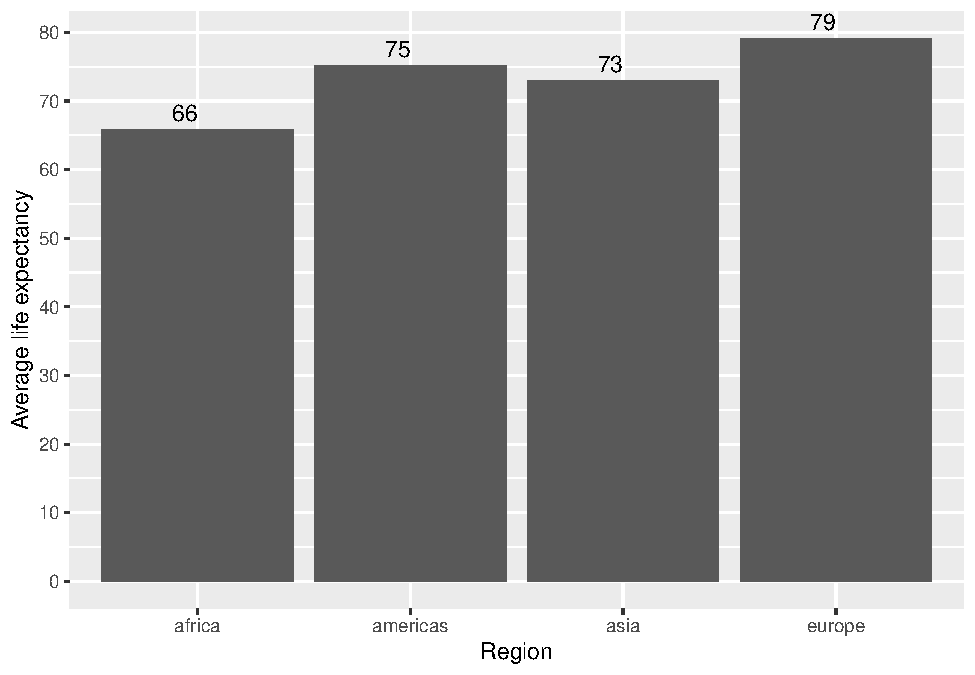
\includegraphics{MTSTIN007_SC_Assingment_2_files/figure-latex/unnamed-chunk-9-1.pdf}

\begin{Shaded}
\begin{Highlighting}[]
\CommentTok{\# title = "Region average life expectancy 2019",}

\CommentTok{\#save plot}
\FunctionTok{ggsave}\NormalTok{(}\StringTok{"region\_avg\_lex\_2019.png"}\NormalTok{)}
\end{Highlighting}
\end{Shaded}

\begin{verbatim}
## Saving 6.5 x 4.5 in image
\end{verbatim}

\begin{Shaded}
\begin{Highlighting}[]
\CommentTok{\#Qtn e}
\NormalTok{country\_split }\OtherTok{\textless{}{-}} \FunctionTok{strsplit}\NormalTok{(lex\_raw}\SpecialCharTok{$}\NormalTok{country, }\StringTok{" "}\NormalTok{)}

\CommentTok{\#get count two word countries}
\NormalTok{two\_word\_countries }\OtherTok{\textless{}{-}} \FunctionTok{sum}\NormalTok{(}\FunctionTok{sapply}\NormalTok{(country\_split, length) }\SpecialCharTok{==} \DecValTok{2}\NormalTok{)}
\NormalTok{two\_word\_countries}
\end{Highlighting}
\end{Shaded}

\begin{verbatim}
## [1] 24
\end{verbatim}

\end{document}
